\section{Analysis}\label{sec:analysis}
\todo{1.5 pages: where the sensor over-reliance comes from, source of the resolution gain, thin objects, failure case, limitations}

% Figure plan: notes/figure_guide.md §2. Qualitative scenes come from recorded dumps only
% (path + md5 in the figure source note) and the selection rule is stated in the caption.

% Fig. dependence (data plot, main evidence for contribution 1).
% Source numbers and provenance: figures/src/make_data_figs.py (fig_dependence).
% Full table: sections/supp_tables.tex (supplementary Table S1).
\begin{figure}[t]
\centering
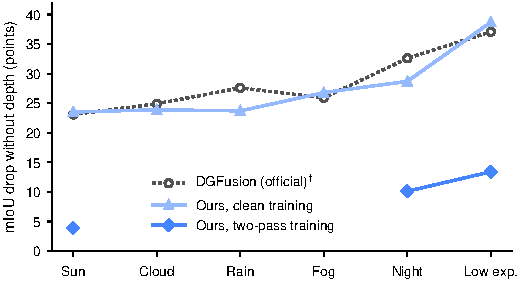
\includegraphics[width=\columnwidth]{figures/fig_dependence.pdf}
\caption{Drop in mIoU when depth is removed, per condition. A model trained only on clean data relies on depth as heavily as DGFusion, whose design adds depth supervision; two-pass training reduces the drop to a third or less with the same architecture. $^{\dagger}$Measured on test; the other curves on val. \todo{re-measure all curves on one split; add the full model and the retrained baselines.}}
\label{fig:dependence}
\end{figure}

% Fig. thin objects. Source: .claude_logs/experiments/analysis/DRN-261018-01/a2_vs_q2_perclass_3seed.csv
% (3 seeds, legal v2 test 1024); plot: figures/src/make_data_figs.py (fig_thin).
\begin{figure}[t]
\centering
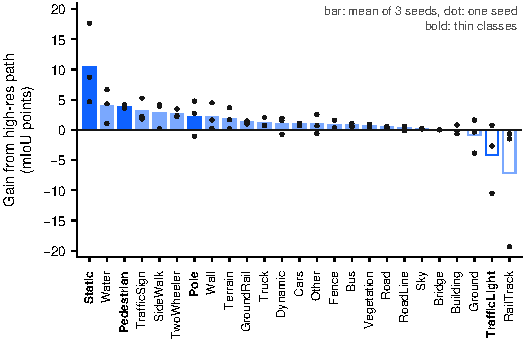
\includegraphics[width=\columnwidth]{figures/fig_thin.pdf}
\caption{Per-class gain of the high-resolution path on DELIVER test, paired by seed (full model minus the same model without the path). Thin classes gain most; TrafficLight and RailTrack lose and vary strongly across seeds (Section~\ref{sec:analysis}). \todo{add zoomed crops of thin objects (Q2 dumps on yeon).}}
\label{fig:thin}
\end{figure}

% Fig. failure case, posters predicted as traffic lights.
% Assets: NAS analysis_logs/a2_tl_fp_scenes_20261022 (4 scenes, README.md has the selection rule).
\begin{figure}[t]
\centering
\phbox{4.2cm}{limitation: posters and signs predicted as traffic light (2 of the 4 recorded scenes; RGB, ground truth, ours, error map)}
\caption{\todo{caption; selection rule from the scene README}}
\label{fig:failure}
\end{figure}
